%%   This file is part of the APS files in the REVTeX 4 distribution.
%%   Version 4.1r of REVTeX, August 2010
%%
%%
%%   Copyright (c) 2001, 2009, 2010 The American Physical Society.
%%
%
\documentclass[aps,prb,reprint,groupedaddress]{revtex4-1}

%\documentclass[aps,pra,twocolumn,groupedaddress]{revtex4-1}
%\documentclass[aps,prb,reprint,superscriptaddress]{revtex4-1}
%%%%%%%%%%%%%%%%%%%%%%%%%%%%%%%%%%%%%%%%%%%%%%%%%%%%%%%%%%%%%%%%%%%%%%%%%%%%%%%%%%%%%%%%%%%%%%%%%%%%%%%%%%%%%%%%%%%%%%%%%%%%
\usepackage{amssymb}
\usepackage{amsthm}
\usepackage{amsmath} 
\usepackage{graphicx}
\usepackage[mathlines]{lineno}% Enable numbering of text and display math
%\linenumbers\relax % Commence numbering lines


%\def\clau#1{\textcolor{ForestGreen}{#1}}
%\def\minor#1{\textcolor{green}{#1}}

\begin{document}

%Title of paper
\title{The role of $4f$ electrons in the stopping power of hafnium}
%Authors and affiliations

%---------------------------Argentina
\author{C. C. Montanari}
\email{mclaudia@iafe.uba.ar}
\affiliation{Instituto de
Astronom\'{\i}a y F\'{\i}sica del Espacio, Consejo Nacional de Investigaciones Cient\'{\i}ficas y
T\'{e}cnicas - Universidad de Buenos Aires, Pabell\'on IAFE, 1428 Buenos Aires, Argentina}%
%\affiliation{Universidad de Tres de Febrero, Sáenz Peña, Buenos Aires, Argentina.}
%------------------------------
\author{A. M. P. Mendez}
\affiliation{Instituto de
Astronom\'{\i}a y F\'{\i}sica del Espacio, Consejo Nacional de Investigaciones Cient\'{\i}ficas y
T\'{e}cnicas - Universidad de Buenos Aires, Pabell\'on IAFE, 1428 Buenos Aires, Argentina}%
%-------------------------------
\author{D. M. Mitnik}
\affiliation{Instituto de
Astronom\'{\i}a y F\'{\i}sica del Espacio, Consejo Nacional de Investigaciones Cient\'{\i}ficas y
T\'{e}cnicas - Universidad de Buenos Aires, Pabell\'on IAFE, 1428 Buenos Aires, Argentina}%
%\affiliation{Universidad de Buenos Aires, Facultad de Ciencias Exactas y Naturales, Departamento de F\'{\i}sica, Ciudad Universitaria, 1428 Buenos Aires, Argentina.}
%----------------------------------------------
\author{J. E. Miraglia}
\affiliation{Instituto de
Astronom\'{\i}a y F\'{\i}sica del Espacio, Consejo Nacional de Investigaciones Cient\'{\i}ficas y
T\'{e}cnicas - Universidad de Buenos Aires, Pabell\'on IAFE, 1428 Buenos Aires, Argentina}%
%---------------------------Chile

\author{P.A. Miranda}
\affiliation{Departmento de F\'isica, Facultad de Ciencias Naturales, Matem\'atica y del Medio Ambiente. Universidad Tecnol\'ogica Metropolitana. 7800002, Chile}
%----------------------------
\author{R. Correa}
\affiliation{Departmento de F\'isica, Facultad de Ciencias Naturales, Matem\'atica y del Medio Ambiente. Universidad Tecnol\'ogica Metropolitana. 7800002, Chile}
\author{J. Wachter}
\affiliation{Departmento de F\'isica, Facultad de Ciencias Naturales, Matem\'atica y del Medio Ambiente. Universidad Tecnol\'ogica Metropolitana. 7800002, Chile}
\author{M. Aguilera}
\affiliation{Departmento de F\'isica, Facultad de Ciencias Naturales, Matem\'atica y del Medio Ambiente. Universidad Tecnol\'ogica Metropolitana. 7800002, Chile}
%-------------------------Lisboa
\author{E. Alves}
\affiliation{Centro de Ci\^{e}ncias e Tecnologias Nucleares, Instituto Superior T\'ecnico, Universidade de Lisboa,
2696-953 Sacav\'{e}m, Portugal}
\affiliation{Instituto de Plasma e Fus\~{a}o Nuclear, Instituto Superior T\'ecnico, Universidade de Lisboa, 2696-953 Sacav\'{e}m, Portugal}
%---------------------------
\author{N. Catarino}
\affiliation{Centro de Ci\^{e}ncias e Tecnologias Nucleares, Instituto Superior T\'ecnico, Universidade de Lisboa,
2696-953 Sacav\'{e}m, Portugal}
%---------------------------
\author{R.C. da Silva}
\affiliation{Centro de Ci\^{e}ncias e Tecnologias Nucleares, Instituto Superior T\'ecnico, Universidade de Lisboa,
2696-953 Sacav\'{e}m, Portugal}



\date{\today}

%=============================================================================================================================================================================================
%=============================================================================================================================================================================================
\begin{abstract}
The stopping power of protons through Hf foil has been studied both experimentally and theoretically. 
The measurements were performed at the Laboratory of Accelerators and X-Ray Diffraction in Lisbon, by using the transmission method on self-supporting stopping material, for (0.6-2.5) MeV protons.
The theoretical developments involved fully relativistic atomic structure calculations for Hf, which required the solution of the Dirac equation. 
The shell-wise local plasma approximation (SLPA) was used to describe the energy transferred to the bound 1s-4f electrons, and the outer four electrons were considered as a free electron gas (FEG). 
 We found the relativistic description of the 4f-shell, and the screening between $4f$ and $5p$ electrons are decisive around the stopping maximum. 
The present theoretical and experimental results have very good agreement in the energy region of the new measurements. 
However, our theoretical stopping cross sections show substantial differences with the semi-empirical models, such as SRIM2013 and ICRU-49, at intermediate to low energies. 
Our calculations suggest the stopping maximum to be larger, and shifted to lower energies, respect to these semi-empirical models. Future measurements below 100 keV would be required to validate our predictions.
\end{abstract}

% insert suggested PACS numbers in braces on next line
\pacs{34.50.Bw} \keywords{Stopping power, Hafnium, Relativistic atomic structure, Transmission method}

\maketitle

%\linenumbers
%=============================================================================================================================================================================================
%=============================================================================================================================================================================================
\section{Introduction}
\label{intro}

For impact energies above a few keV/amu, mono-energetic charged particles penetrating a foil of any material lose their energy through a series of consecutive inelastic collisions, mainly with target electrons \cite{Chu01,Sigmund}. 
The information given by the energy loss process is essential not only to have a better knowledge of the phenomena behind the fundamental interactions but also because it plays an important role in many applied fields such as materials science, nuclear physics, ionic implantation, and radiotherapy \cite{Sigmund,Schardt}. 
Experimental data in ion mean energy loss per unit path $S(E)$ is of crucial relevance to check the reliability of semi-empirical models and to determine some key parameters \cite{Diwan,Damache04,Damache02}. 
However, often, the experimental data available is rather scarce, which is troublesome when the material under study corresponds to an element of low occurrence on the Earth's upper crust, such as Hf.

So far, only one experimental work has been published regarding the stopping power cross section of pure hafnium for protons \cite{Sirotinin}, while more attention has been recently given to studies involving hafnium oxide because of its practical use \cite{Abril,Behar,Primetzhofer}. 
It is well known that significant attention has been paid in recent years to transition metal-oxides such as HfO$_2$ because of their potential as alternative gate dielectrics to replace SiO$_2$ for the future generation of nano-electronics with less than 45 nm gate length \cite{Choi,Robertson}. 
Some important physical properties of the above mentioned metal-oxide films depend on its thickness, which is often measured by using Rutherford Backscattering Spectrometry \cite{Alfassi01, Tesmer01}, a method that relies heavily on the determination of the stopping power of ion beams in the material of interest.

In this study, we report experimental stopping power cross section values over the incident energy range (0.6-2.5) MeV for protons crossing self-supported Hf thin-film by using the transmission method.
We aim not only to upgrade stopping power data compilations \cite{HPaul03,mondim17} but also to provide useful information about the processes governing the slowing down of protons in multi-electronic targets. 
In the rare earth metals, the $4f$ electrons play a relevant role in the stopping power, being the first shell of bound electrons below the conduction band. As already noted \cite{Roth17}, the free electron gas (FEG) shows unexpected behavior in these elements, which casts doubts on its proper description. With Hf, we found the contribution of the 4f-shell decisive even at impact energies around the stopping maximum, as shown later.

The theoretical approach implemented in this work uses the shell-wise local plasma approximation (SLPA) \cite{mon13} to describe the energy transferred to the bounds 1s-4f electrons, and two different models for the FEG: the screened potential with cusp condition model (SPCC) \cite{mon17}, which is non-linear binary formalism; and the Mermin-Lindhard dielectric formalism (ML) \cite{Mermin}, for energies around the stopping maximum and above. 
Our model requires the relativistic description of the wave functions and binding energies of Hf \cite{mendez2019}, where we consider 4 electrons per atom in the FEG. 
The 14 electrons occupying the 4f subshell of Hf makes up the main contribution to the stopping below the FEG, which causes the cross sections to be very sensitive to a good description of this shell. 
The screening between the 4f and 5p electrons has been considered, and it has been found to play a major role within the SLPA predictions.

%The theoretical approach used in this work requires the relativistic wave functions and binding energies of Hf, and considering 4 electrons per atom in the free electron gas (FEG) \cite{mendez2019}. The shell-wise local plasma approximation (SLPA) \cite{mon13} was employed to describe the energy transferred to the bound 1s-4f electrons, and two different models for the FEG: the screened potential with cusp condition model (SPCC) \cite{mon17}, which is non-linear binary formalism; and the Mermin-Lindhard dielectric formalism (ML) \cite{Mermin}, for energies around the stopping maximum and above.  On the other hand, Hf has the extra interest of the filled $4f$-subshell (with 14 electrons) as the main contribution below the FEG, causing the stopping cross sections to be very sensitive to a good description of this shell. The screening among the $4f$ and $5p$ electrons has been considered and found to play a major role within the SLPA calculations.

The experimental details and data are given in Section \ref{experiment}, while the theoretical method is explained in Section \ref{theory}. Finally, our theoretical approach and experimental measurements are compared to the available experimental values \cite{Sirotinin}, the ICRU-49 calculations \cite{ICRU49}, and the SRIM-2013 package \cite{Ziegler01}. Conclusions and discussions are given in Section \ref{conclusion}.

%=============================================================================================================================================================================================

\begin{figure}[!t]
\centering
\includegraphics[width=9cm]{Fig01.eps}
\caption{RBS spectrum for $E_{\mathrm{avg}} = 921.1$ keV protons on hafnium sample, which is subsequently used to determine the energy loss in the foil.}
\label{F01}
\end{figure}

%=============================================================================================================================================================================================

\section{Experimental arrangements}
\label{experiment}
\subsection{Accelerator and scattering Chamber}
The procedure carried out to obtain the stopping power data in this work is essentially the same as the one detailed in Ref. \cite{Miranda01}. However, the present measurements were performed at the IST/LATR (Laboratory of Accelerators and X-Ray Diffraction) in Lisbon. This facility uses a 2.5 MV Van de Graaff accelerator to deliver $^1$H$^+$ primary ion beams through a series of electrostatic lenses and collimators onto a thin Au/SiO$_2$ sample which is used as a scattering center. This sample was placed in the center of an RBS/C scattering chamber, where a high vacuum (pressure of $\sim$10$^{-6}$ Torr) was maintained during the measurements. The beam current on the sample was kept at around 5.0 nA to attain sufficient statistics in each particle spectrum. 
By using a beam spot of about 1.0 mm in diameter, a solid angle of 11.4 msr was attained. The overall energy resolution (FWHM) of the detection system was about 15 keV relative to 5.486 MeV alpha particles from a $^{241}$Am source.

%---------------------------------------------------------------------------------------------------------------------------------------------------------------------------------------------
\subsection{Target}
The stopping material under analysis was a hafnium foil with a nominal thickness of 1.0 $\mu$m and 99.95\% purity, which was supplied by Lebow Company \cite{Lebow}. However, a more precise thickness value was achieved by measuring the energy loss of alpha particles coming from a calibrated ($^{239}$Pu, $^{241}$Am, $^{244}$Cm) source. From the alpha spectra with and without the Hf foil interposed, the characteristic energy shift $\delta$E was measured and then combined with the stopping power for 5.486 MeV alphas on hafnium (55.69 eV/$10^{15}$ at/cm$^2$) found in Ref.\cite{Ziegler01} to obtain an areal density of ($4.13\pm0.21$)$\times 10^{19}$ at/cm$^2$, which corresponds to a thickness of $0.920\pm0.046 \mu$m.

%---------------------------------------------------------------------------------------------------------------------------------------------------------------------------------------------
\subsection{Energy loss measurement}
Once the beam impinges on the Au/SiO$_2$ sample, protons are backscattered towards a Si surface barrier detector located at 140$^{\circ}$ relative to the initial beam direction. Fig.\ref{F01} shows two-particle spectra, where ion energies $E_2$ and $E_1$ are associated to a placed and removed hafnium sample, respectively. Both energy distributions were fitted by Gaussian functions to obtain the mean energy and width (FWHM) of the peaks \cite{Sun01}, and from the difference between these two peak positions in the spectrum, the total energy loss $\Delta E = (E_1 - E_2)$ in the foil was calculated. As established in previous studies \cite{Miranda01, Damache02}, the experimental stopping power cross sections $\varepsilon (E) $ are determined at some mean energy $E_{\mathrm{avg}}$ by measuring the ion energy losses $\Delta E$ within the investigated Hf foil, which has a mean thickness denoted by $\Delta x$. In this way, only when the energy loss fraction $\Delta E/E_{\mathrm{avg}}$ across the Hf foil is not exceeding 20\% it is possible to define the stopping cross section by \cite{Raisanen01,Schulz01}
\begin{equation}\label{eq:stcross}
 \varepsilon (E) = \frac{S(E)}{N} = -\frac{dE}{N dx} \approx -\frac{\Delta E}{N \Delta x}\,,
\end{equation}
where $N$ denotes the atomic number density (atoms cm$^{-3}$) of the material under study. When this condition was not fulfilled, a small correction to the mean energies $E_{\mathrm{avg}}$ was applied in order to account for the nonlinear dependence on ion energy of stopping powers \cite{Chilton,Rajatora}.

\section{Theoretical Method} 
\label{theory}
The energy loss of ions in metal targets responds to different physical mechanisms, depending on the impact ion velocity. At low velocities, the binary collisions are responsible for the loss of energy by the ion. The main contribution is the ionization of electrons in the metal conduction band, which is well approximated by a free electron gas (FEG) of Fermi velocity $v_F$. Above a certain velocity (i.e. $v\geq 1.5 \ v_F$), not only binary but also collective excitations (plasmons) are possible \cite{mon17}. Moreover, at high energies, both the FEG and the bound electrons contribute to the stopping power. The method used in this work combines a description for the interaction with the valence (or conduction) electrons as a FEG, and a different one for the interaction with the bound electrons.

We used the SPCC model \cite{mon17} to describe the stopping power of low velocity charged particles in the FEG. The model relies on a non-perturbative binary collisional approximation. The SPCC \cite{mon17} is based on a screened central potential with a cusp condition of the electronic density close to the projectile. This model proved to give a good description of the induced electron density even for negative projectiles \cite{mon17} and reproduces the low-velocity proton-antiproton differences in the stopping power (Barkas effect). The SPCC formalism only depends on the Wigner-Seitz radio, $r_S$, which is a measure of the electronic density of the FEG. For metals of well-known $r_S$ values, the SPCC describes correctly the low energy experimental stopping data \cite{mon17}, agreeing with the DFT results by Echenique and coworkers \cite{eche81,nagy89} at $v=0$. 

Hafnium ($Z=72$, [Xe] $4f^{14} \ 6s^2 \ 5d^2$) belongs to the first group of transition metals, with  4 electrons as FEG (theoretical $r_S=2.14$ a.u.) and $1s-4f$ electrons bound. We compared the computed $r_S$ with the experimental value obtained from the measured energy loss function by Lynch \textit{et al} \cite{lynch75}. The experimental plasmon energy of Hf is $\hbar\omega_P \approx 15.8$ eV, with a width at half maximum of $\delta \approx 4.4$ eV, and $r_S \approx 2.07$ a.u. \cite{lynch75}. The difference of less than $5\%$ between theoretical and experimental $r_S$ assess Hf as a canonical target\cite{mon17}.

Above certain impact velocity, the plasmon contribution is important (i.e. around and above the stopping maximum). An interesting value for our analysis is the minimum impact velocity to excite
plasmons, $v_P$. In the dielectric formalism, this value can be obtained as $v_P\ \approx \ v_F[1+(3 \pi\ v_F)^{-1/2} ]$ \cite{suppression}. To describe the energy loss considering collective and binary excitation, we resort to the ML dielectric formalism \cite{Mermin}, which is a linear response, perturbative approximation, so it depends on the square of the ion charge. In this formalism, the response of target electrons to the ion passage is described through the quantum dielectric function, depending on the characteristic $r_S$ and $\delta$ parameters of the FEG. 

%----------------------------------------------------------------------
\begin{figure*}[!t]
\centering
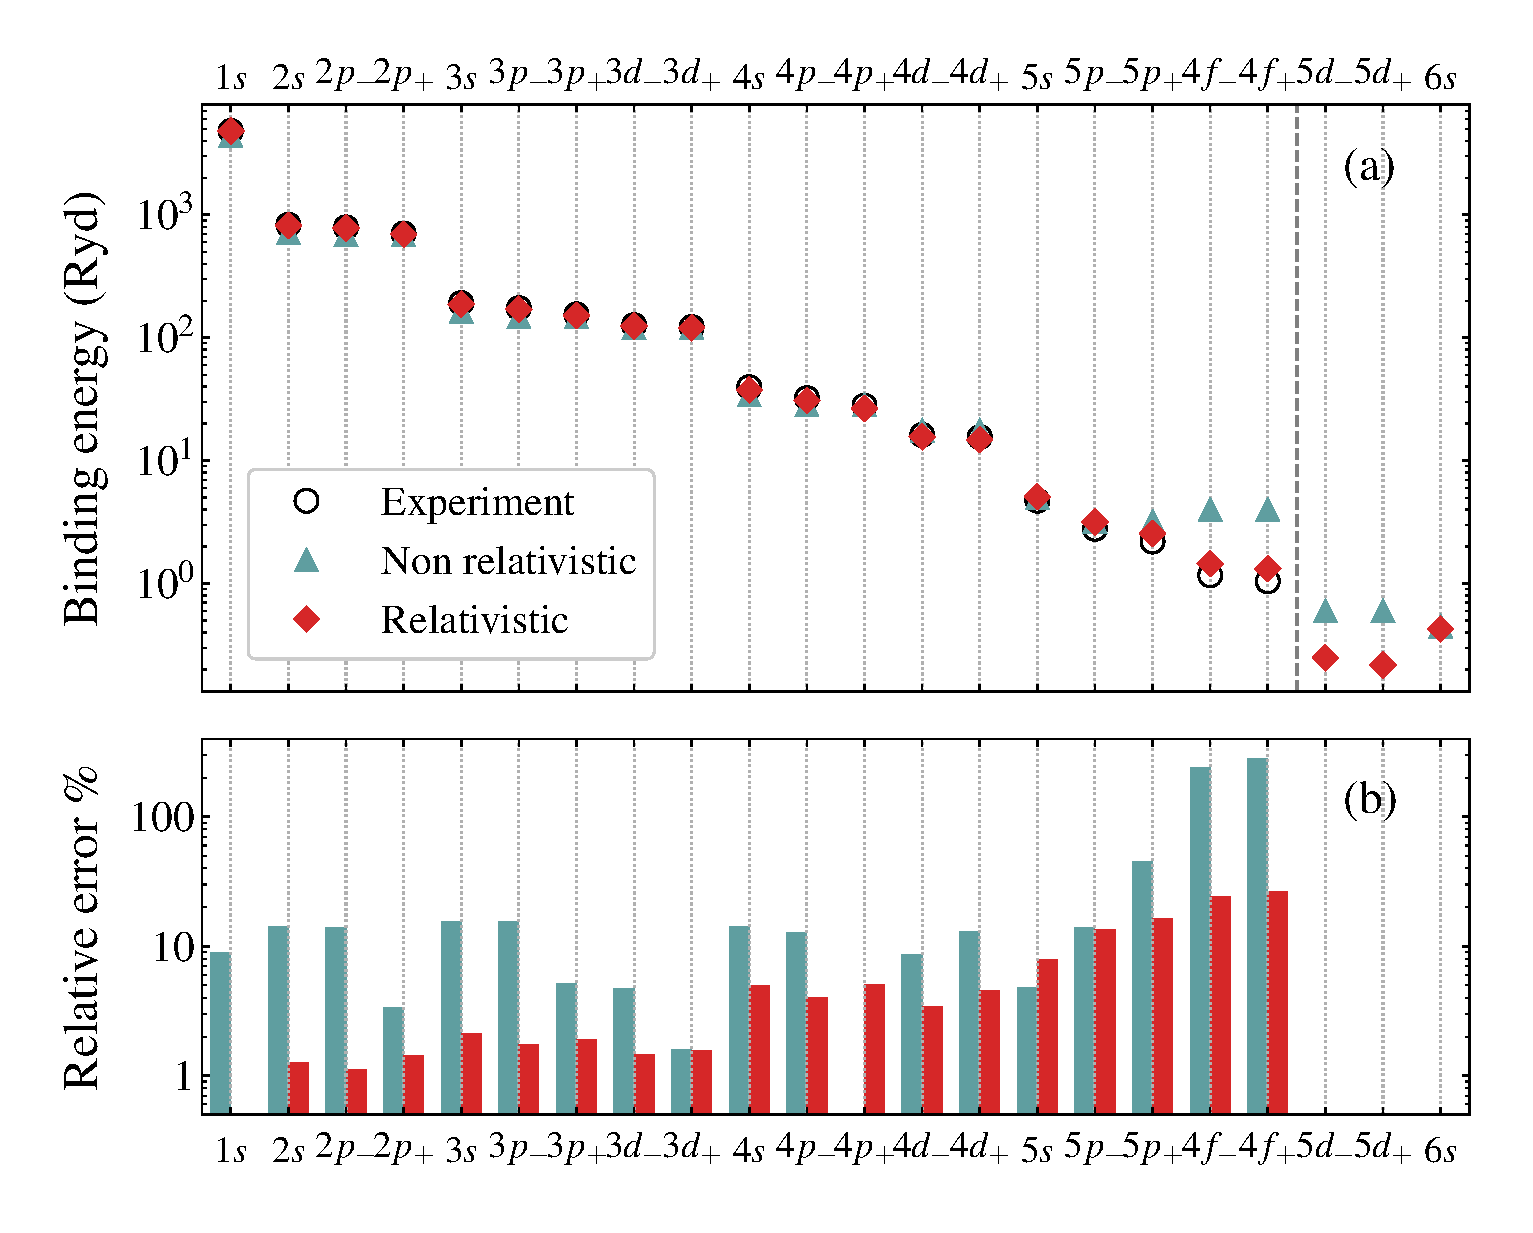
\includegraphics[width=11.cm]{Hf_bindener_bar.eps}
% 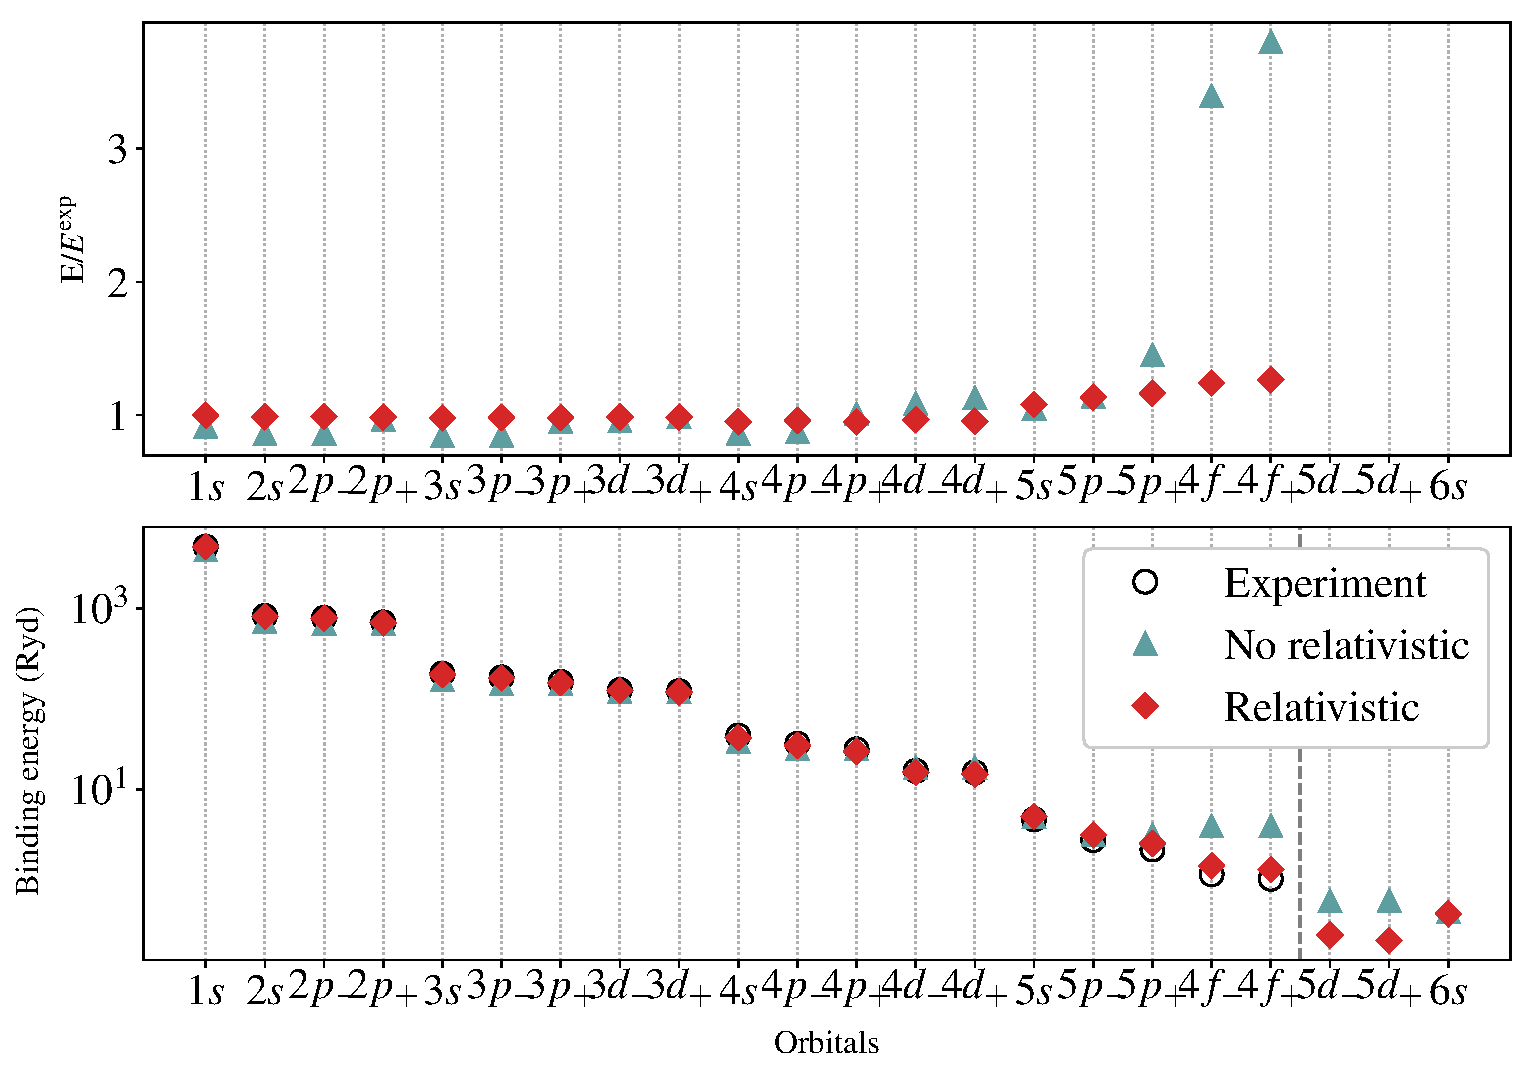
\includegraphics[width=13.cm]{Hf_bindener_ratio.eps}
\caption{(a) Binding energies of Hf. Non relativistic and relativistic calculations are given with filled symbols.  Experimental measurements for solids\cite{williams1995} are depicted with hollow circles. (b) Corresponding relative errors respect to experimental data.}
\label{Binding_E}
\end{figure*}
%------------------------------------------------------------------------

For the stopping power due to bound electrons, the SLPA \cite{mon17,mon13} is employed. It is worth mentioning that the only inputs for the SLPA are the space-dependent densities of each shell in the ground state, and their binding energies. Collective processes and screening among electrons are included. Hafnium is a relativistic target, therefore the wave functions and binding energies must be obtained as solutions of the Dirac equation\cite{mendez2019}.

To asses the importance of the relativistic description of the bound electrons, Figure \ref{Binding_E} (a) shows non relativistic and relativistic binding energies $E_{nl\pm}$, where $\pm=j\pm1/2$.
We compare our results with experimental measurements on solid Hf \cite{williams1995} from $1s$ to $4f_{\pm}$. We notice that not only the most inner shells require relativistic calculations, but also the outer $5p$ and $4f$ shells. Figure \ref{Binding_E} (b) presents the relative error of non relativistic and relativistic energies with respect to the experimental data in logarithmic scale. This figure shows very clearly the disability of non-relativistic calculations to describe the experimental data, which surprisingly worsens from the inner to the outer shells. 
%It is clear in this figure the disability of non-relativistic binding energies to describe the experimental data, which surprisingly worsens from the inner to the outer-shells.
%We used here the theoretical binding energies and wave functions of Hf calculated in \cite{mendez2019}. 
%The present theoretical description of Hf considers a FEG of $r_S=2.14$ and 1s-4f electrons as bound. 


%The relativistic results for binding energies and wave functions in \cite{mendez2019} 
Our relativistic binding energies present spin-orbit split. However, in total stopping power where the initial state of the excited electron is not measured, the quantum uncertainty in energy $\Delta E$ melts this split. The criteria $\Delta E\Delta t \geq \hbar /2$ merges the energies  $E_{nl+} - E_{nl-}$ for sufficiently small values of $\Delta t$ (the collisional mean-time). In fact, at sufficiently high impact velocity we can expect all target electrons to respond together to the ion passage \cite{lindhard53,chu72}. As in \cite{mon09}, the collisional time was estimated as follows $\Delta t \approx \langle r_i\rangle/v$, with $\langle r_i\rangle$ and $v$ being the orbital mean radio and impact velocity, respectively. 



%--------------------------------------------------------------------------------
\begin{figure*}[!t]
\centering
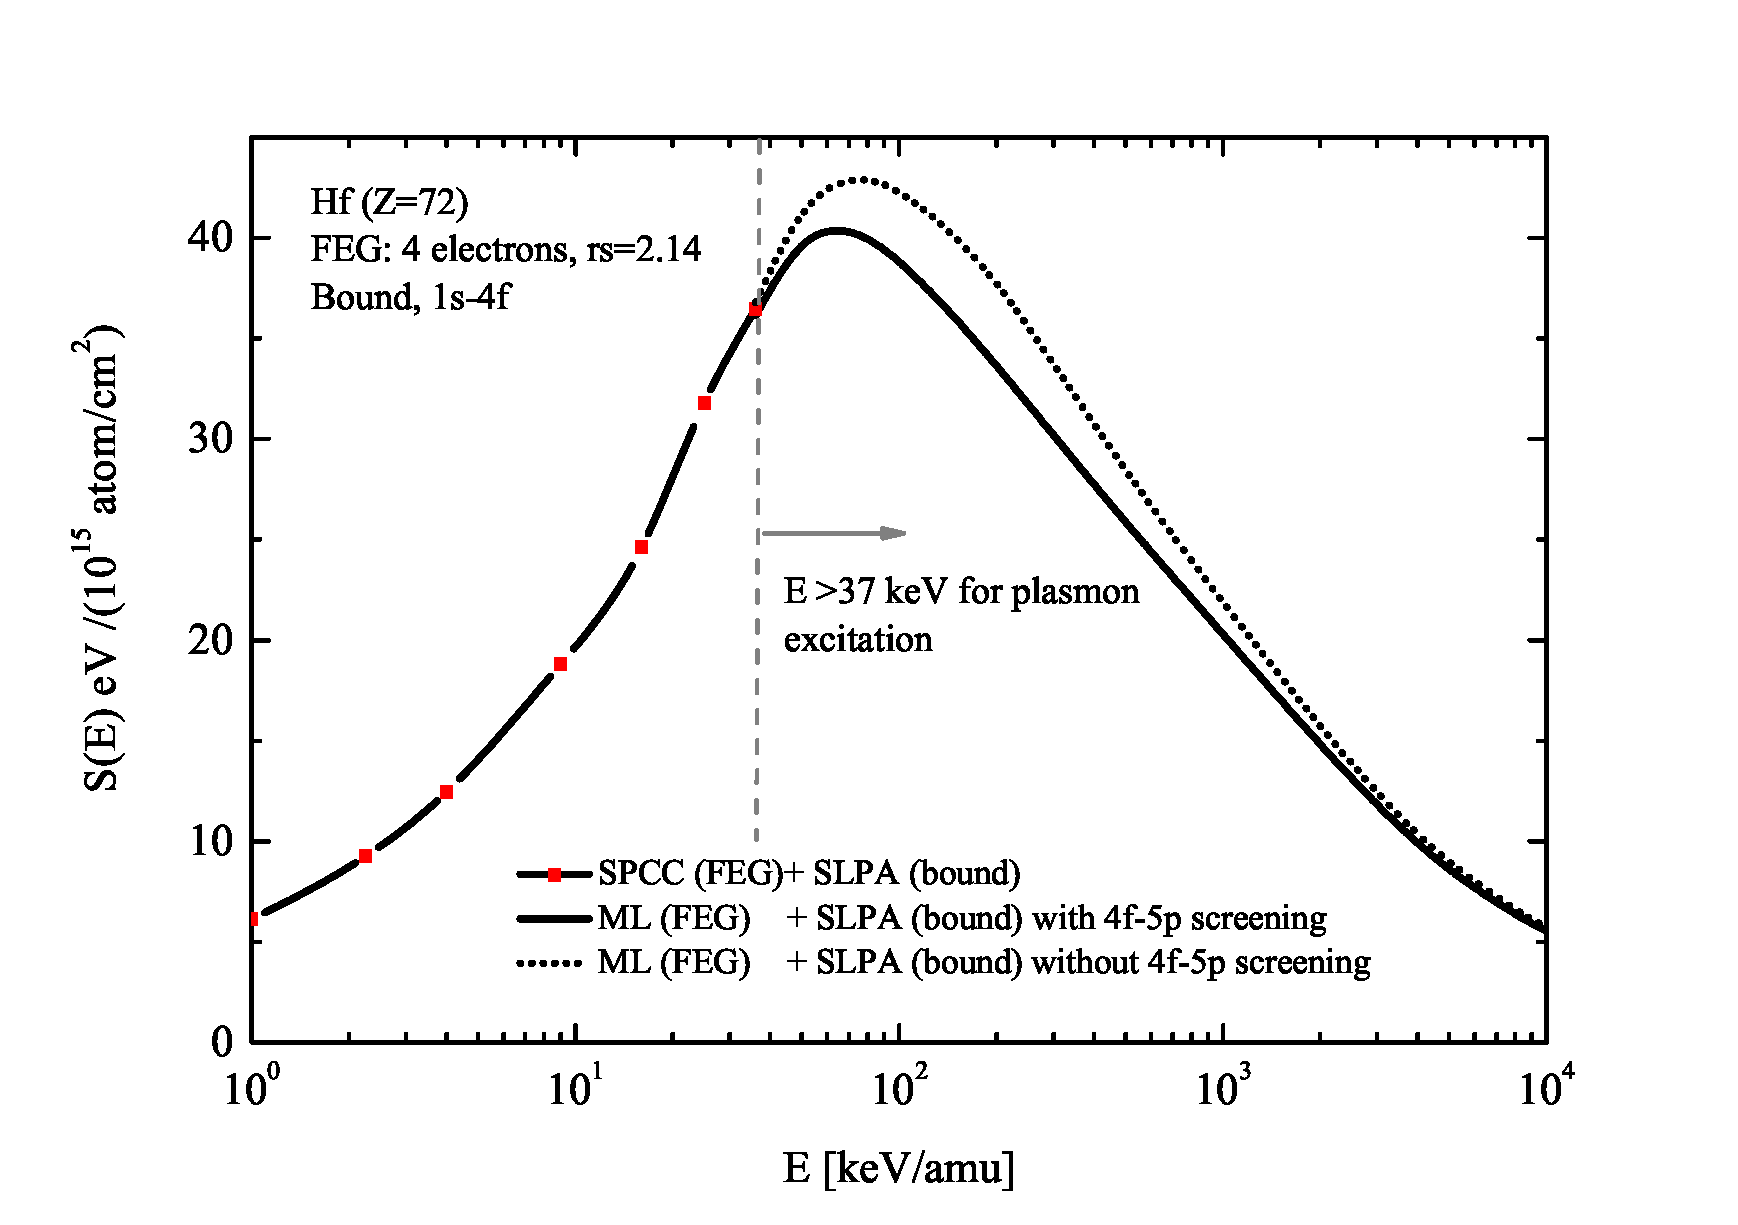
\includegraphics[width=13.cm]{Fig02.eps}
\caption{Theoretical total stopping cross sections of protons in afnium adding FEG and bound $1s$-$4f$ contributions, as mentioned in the inset. The vertical grey dashed-line indicates the energy above which plasmon excitation is possible. %The FEG calculations employ the SPCC model at low energies (no plasmon excitation) and the ML formalism (includes plasmon excitation). 
The SLPA calculations for $1s$-$4f$ bound electrons with and without $5p-4f$ screening give different total stopping values, displayed with solid and dotted lines, respectively.}
\label{slpa4f}
\end{figure*}
%========================================================================================

The SLPA calculates the contribution of each subshell of bound electrons to the total stopping cross sections. We found that for every sub-shell of Hf, at the impact energy at which this sub-shell began to contribute, the spin-orbit split was unresolved.  Then the $nl$-electrons should be considered together, responding to the ion passage as a single gas of electrons with density $\delta_{nl}(r)$ and a mean binding energy $E_{nl}$. This is important within the SLPA calculations because of the screening among electrons of the \textit{same} binding energy. For example, the $4f_{-}$ and $4f_{+}$ of Hf can only be resolved for impact energies $E<0.05$ keV, but the contribution of $4f$ to the total stopping is negligible if $E<40$ keV. Moreover, the $5p$ and $4f$ electrons of Hf are very close in energy ( $\Delta E_{5p-4f} \approx 1 a.u.$ \cite{mendez2019}) %merges them 
and react together for impact energies $E>40$ keV (inter-shell screening).

%================================================================================
\begin{figure*}[!t]
\centering
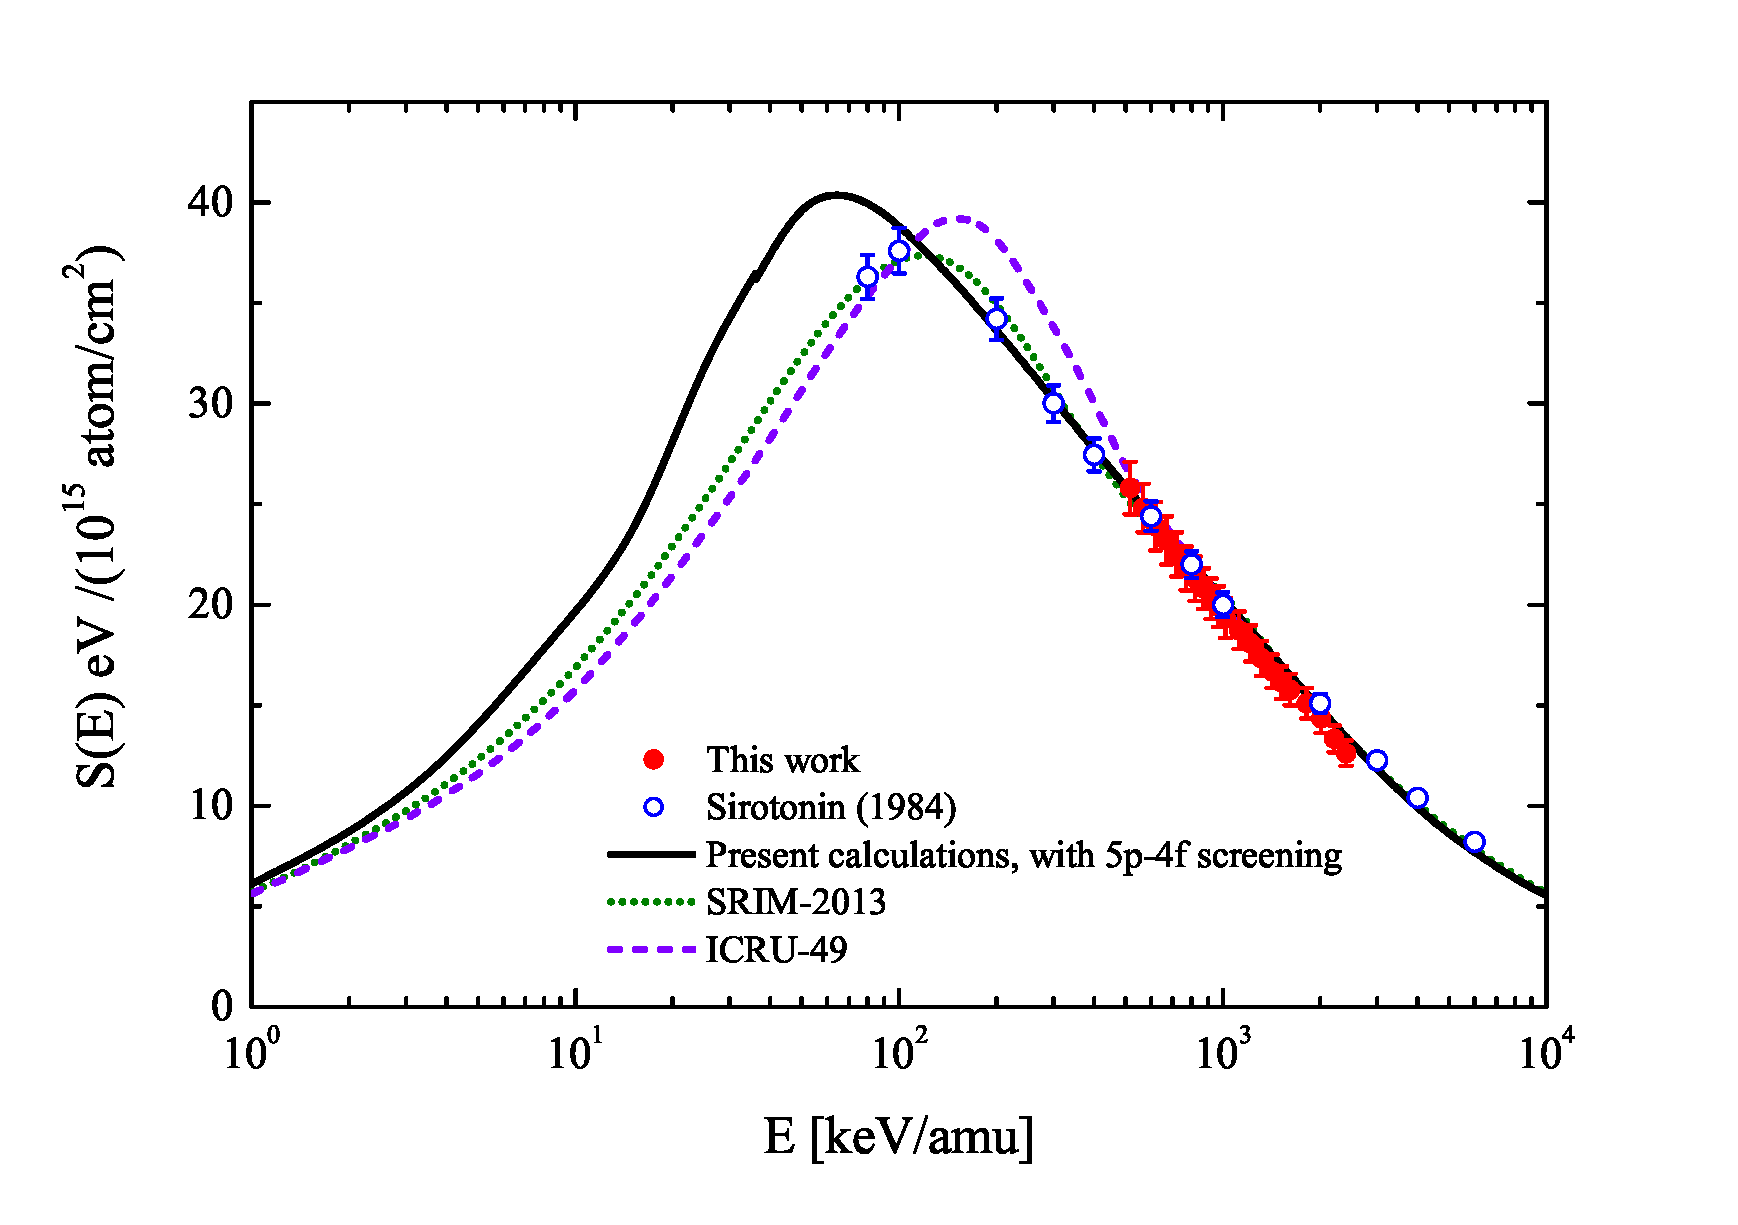
\includegraphics[width=13.0cm]{Fig03.eps}
\caption{Stopping power cross section of hafnium for protons. Symbols: solid circles, present values; open circles, previous data \cite{Sirotinin}. Curves: Black solid-line, present full theoretical results with $4f$-$5p$ screening; violet dashed-line, values from ICRU-49 \cite{ICRU49}, and green dotted line, SRIM-2013 \cite{Ziegler01}.}
\label{F03}
\end{figure*}
%=============================================================================================================================================================================================

In figure \ref{slpa4f} we display the present theoretical stopping cross section of Hf for protons with and without the $5p-4f$ screening. We added the FEG and the bound electron contributions as explained above. The minimum energy for plasmon excitation was estimated as $37$ keV. We used the non-perturbative SPCC model for impact energies $E \leq 37$ keV, and the perturbative ML calculation above this energy. %The range of validity of the perturbative model below 100 keV is arguable, however the asymetric $Z_{ion}/Z_{target}$ relation is clear. 
%The importance of the 4f-5p screening is signed with arrows in this figure. 
Clearly, considering $5p-4f$ electrons as a single group of 20 electrons with screening among them gives lower stopping values than the addition of the separate $5p$ and $4f$ contributions. This is a shell correction that can only be considered within a many electron model such as the SLPA.

%=============================================================================================================================================================================================
\section{Analysis of the results and discussion}
\label{discussion}

The present data and theoretical results are displayed in table \ref{table01}, and figure \ref{F03}. As can be seen in Table~\ref{table01}, an overall relative uncertainty of around 5$\%$ was achieved for the experimental stopping power values, mainly due to the uncertainty in the hafnium foil thickness. %A good agreement in the whole energy range is found between our new data and the previous measurements made by Sirotinin \textit{et al.} \cite{Sirotinin}, as depicted in Fig.~\ref{F03}. Also shown in the same figure are our theoretical stopping cross sections together with the semi-empirical SRIM-2013 curve \cite{Ziegler01} and the suggested values by the ICRU-49 report \cite{ICRU49}. 

%-----------------TABLE--------------------------------------------------------------------------
\begin{table*}[!t]
\centering
\caption{Stopping power values S$_{exp}$ of hafnium for protons measured in this work. $\Delta$E/E values are also shown.
\label{table01}}

\vspace{0.2cm}

\begin{ruledtabular}
\begin{tabular}{ccc|ccc|ccc} %\hline\hline
E$_{avg}$	&S$_{exp}$			&$\Delta$E/E	&E$_{avg}$	&S$_{exp}$			&$\Delta$E/E	&E$_{avg}$	&S$_{exp}$			&$\Delta$E/E\\
keV		&eV/(10$^{15}$ at/cm$^2$)	&$\%$		&keV		&eV/(10$^{15}$ at/cm$^2$)	&$\%$		&keV		&eV/(10$^{15}$ at/cm$^2$)	&$\%$\\ \hline
516,6	&	25,8	$\pm$	1,3	&	20,5	&	1170,3	&	18,25	$\pm$	0,91	&	6,4	&	1813,4	&	15,10	$\pm$	0,76	&	3,4	\\
567,8	&	24,8	$\pm$	1,2	&	17,9	&	1220,0	&	18,08	$\pm$	0,90	&	6,1	&	1862,7	&	14,79	$\pm$	0,74	&	3,3	\\
618,8	&	23,9	$\pm$	1,2	&	15,8	&	1269,6	&	17,57	$\pm$	0,88	&	5,7	&	1912,0	&	14,21	$\pm$	0,71	&	3,0	\\
669,6	&	23,2	$\pm$	1,2	&	14,2	&	1319,2	&	17,32	$\pm$	0,87	&	5,4	&	1961,2	&	14,46	$\pm$	0,72	&	3,0	\\
720,1	&	22,5	$\pm$	1,1	&	12,8	&	1368,8	&	17,15	$\pm$	0,86	&	5,1	&	2010,4	&	14,34	$\pm$	0,72	&	2,9	\\
770,5	&	21,8	$\pm$	1,1	&	11,6	&	1418,3	&	16,69	$\pm$	0,83	&	4,8	&	2059,6	&	13,76	$\pm$	0,69	&	2,7	\\
820,8	&	21,3	$\pm$	1,1	&	10,7	&	1467,8	&	16,43	$\pm$	0,82	&	4,6	&	2108,8	&	13,78	$\pm$	0,69	&	2,7	\\
871,0	&	20,8	$\pm$	1,0	&	9,8	&	1517,2	&	16,13	$\pm$	0,81	&	4,4	&	2158,0	&	13,70	$\pm$	0,69	&	2,6	\\
921,1	&	20,3	$\pm$	1,0	&	9,1	&	1566,7	&	16,04	$\pm$	0,80	&	4,2	&	2206,5	&	13,33	$\pm$	0,67	&	2,5	\\
971,1	&	19,9	$\pm$	1,0	&	8,4	&	1616,0	&	15,77	$\pm$	0,79	&	4,0	&	2256,4	&	13,27	$\pm$	0,66	&	2,4	\\
1021,0	&	19,33	$\pm$	0,97	&	7,8	&	1665,4	&	15,51	$\pm$	0,78	&	3,8	&	2305,5	&	13,07	$\pm$	0,65	&	2,3	\\
1070,8	&	19,03	$\pm$	0,95	&	7,3	&	1714,8	&	15,46	$\pm$	0,77	&	3,7	&	2354,7	&	12,91	$\pm$	0,65	&	2,2	\\
1120,6	&	18,73	$\pm$	0,94	&	6,9	&	1764,1	&	14,93	$\pm$	0,75	&	3,5	&	2403,8	&	12,61	$\pm$	0,63	&	2,2	\\ \\ %\hline
\end{tabular}
\end{ruledtabular}
\end{table*}


There is good agreement between the present theoretical results, the new data in Table~\ref{table01}, and also with previous data by Sirotinin \cite{Sirotinin}, except for the lowest energy measurement at 80 keV. It is interesting that our full theoretical curve differs from SRIM-2013 one for impact energies below 100 keV. We obtain a stopping maximum around 40 $10^{-15}$ eV cm$^2$/atom  at 65 keV. Instead, following the up-to-now only set of data \cite{Sirotinin}, SRIM-2013 suggests a lower stopping maximum %of 37.4 $10^{-15}$ eV cm$^2$/atom 
at impact energy of 115 kev. It is worth to mention that similar theoretical results using the experimental $r_S=2.07$ a.u. instead of the theoretical $r_S=2.14$ a.u. give the stopping maximum at the same impact energy but $4\%$ higher. Future experiments for
impact energies below 100 keV would be important to complete this study.


%=============================================================================================================================================================================================
%=============================================================================================================================================================================================
\section{Conclusion}
\label{conclusion}
In this work, we have used the transmission method to experimentally determine stopping power cross section values for (0.6-2.5) MeV protons incident on self-supporting Hf foils with an overall uncertainty of around 5\%. Additionally, we calculated values extracted from the theoretical framework that involved the relativistic wave functions and binding energies of Hf, and considered 4 electrons per atom in the free electron gas. The shell-wise local plasma approximation was employed to describe the energy transferred to the bound 1s-4f electrons, and two different models for the FEG: the screened potential with cusp condition (SPCC model) for energies below that of the plasmon excitation, and the Mermin-Lindhard dielectric formalism, for energies around the stopping maximum and above. Present theoretical stopping cross sections cover an extensive energy range from 1 keV/amu-10 meV/amu.

%Our results have been confronted to both experimental values found in the literature and semi-empirical results. 
At high impact energies, the new stopping  measurements are in good agreement with our theoretical results, and also with already published experimental data and semi-empirical values calculated by means of SRIM-2013 and ICRU-49.  However, we call the attention that around the stopping maximum and at lower impact energies the difference between our full-theoretical results and SRIM is substantial. To our knowledge, these are the first theoretical calculations of stopping in Hf taking into account the atomic relativistic effect.
%for energies around and below the stopping maximum, the present full-theoretical results clearly differ from semiempirical SRIM values, which are based on previous data. 
Future experiments for impact energies below 100 keV would be important to complete this study.
%=======================================================================================================================================
\begin{acknowledgments}
This work was funded by VRAC Grant Number L1-17 of Universidad Tecnol\'ogica Metropolitana, Chile; also by the Consejo Nacional de Investigaciones Científicas y Técnicas (CONICET), the Agencia Nacional de Promoción Científica y Tecnológica (ANPCyT), and Universidad de Buenos Aires (UBA), of Argentina.

The authors gratefully acknowledge the invaluable contribution of F. Baptista from ITN/IST-UTL, Sacav\'{e}m, Portugal for his constant availability. 
\end{acknowledgments}

%=======================================================================================================================================
%  references
\begin{thebibliography}{00}
%============================================================================================================================
%Fundamentals of Stopping Power and Energy Loss processes
\bibitem{Chu01} W.K. Chu, J.W. Mayer, M.A. Nicolet (Eds.) Backscattering Spectrometry, Academic Press, New York, 1978.
\bibitem{Sigmund} P. Sigmund, ''Particle Penetration and Radiation Effects. General Aspects and Stopping of Swift Point Charges``.
Springer Series in Solid-State Sciences, Vol. 151, Springer, Berlin (2006).
\bibitem{Schardt} D. Schardt, T. Els\"asser, D. Schulz-Ertner, Rev. Mod. Phys. \textbf{82},  383-425 (2010).
\bibitem{Diwan} P.K. Diwan, S. Kumar, Nucl. Instr. and Meth. B \textbf{359}, 78-84 (2015).
%\bibitem{Damache01} D. Moussa, S. Damache and S. Ouichaoui, Nucl. Instr. and Meth. \textbf{B} 343,  44-47 (2015).
\bibitem{Damache02} D. Moussa, S. Damache and S. Ouichaoui, Nucl. Instr. and Meth. B \textbf{268}, 1754-1758 (2010); \textbf{343},  44-47 (2015).
%\bibitem{Damache03} S. Damache, S. Ouichaoui, D. Moussa and A. Dib, Nucl. Instr. and Meth. \textbf{B} 249,  22-25 (2006).
\bibitem{Damache04} S. Damache, S. Ouichaoui, A. Belhout, A. Medouni and I. Toumert, Nucl. Instr. and Meth. B \textbf{225}, 449-463 (2004).
%============================================================================================================================
%% Use of Hafnium and Stopping Power of Hafnium
\bibitem{Sirotinin} E.I. Sirotinin, A.F. Tulinov, V.A. Khodyrev, V.N. Mizgulin, Nucl. Instr. and Meth. B \textbf{4}, 337-345 (1984).
\bibitem{Abril} I. Abril, M. Behar, R. Garc\'a Molina, R.C. Fadanelli, L.C.C.M. Nagamine, P.L. Grande, L. Sch\"unemann, C.D. Denton, N.R. Arista, E.B. Saitovich,
Eur. Phys. J. D \text{54}, 65-70 (2009).
\bibitem{Behar} M. Behar, R.C. Fadanelli, I. Abril, R. García-Molina, C.D. Denton, L.C.C.M. Nagamine, N.R. Arista, Phys. Rev. A \textbf{80},  062901 (2009).
\bibitem{Primetzhofer} D. Primetzhofer, Nucl. Instr. and Meth. B \textbf{320}, 100-103 (2014) .
%============================================================================================================================
% Why Hafnium is so important:
\bibitem{Choi} J.H. Choi, Y. Mao, J.P. Chang, Mat. Sci. Eng. R \textbf{72}, 97-136 (2011) .
\bibitem{Robertson} J. Robertson, R.M. Wallace, Mat. Sci. Eng. R \textbf{88}, 1-41 (2015) .
%============================================================================================================================
%Importance of Stopping Power for Ion Beam Analysis
\bibitem{Alfassi01} Z.B. Alfassi, "Non-destructive elemental analysis", Blackwell Science Ltd. (2001).
\bibitem{Tesmer01} J.R. Tesmer, M. Nastasi, J.C. Barbour, C.J. Maggiore and J.W. Mayer, ''Handbook of Modern Ion Beam Material Analysis``, Materials Research Society (1995).
\bibitem{HPaul03} https://www-nds.iaea.org/stopping/.
\bibitem{mondim17} C.C. Montanari, and P. Dimitriou, Nucl. Instr. and Meth. B \textbf{408},  50-55 (2017).
\bibitem{Roth17} D. Roth, B. Bruckner, M. V. Moro, S. Gruber, D. Goebl, J. I. Juaristi, M. Alducin,R. Steinberger, J. Duchoslav, D. Primetzhofer, and P. Bauer1, Phys. Rev. Lett \textbf{118}, 103401 (2017)

%============================================================================================================================
%Semi-empirical and Theoretical approach

\bibitem{mendez2019} A.M.P. Mendez, C.C. Montanari, D.M. Mitnik, %\textit{Relativistic atomic structure calculations of heavy targets for inelastic collisions}, 
Nucl. Instrum. Meth. B \textbf{460}, 114-118 (2019) .
\bibitem{williams1995}
G. Williams in http://xdb.lbl.gov/Section1/Sec\_1-1.html
\bibitem{mon13} C.C. Montanari and J.E. Miraglia, Adv. Quant. Chem. \textbf{65}, edited by Dz. Belkic (Elsevier, Amsterdam, 2013), Chap. 7, pp. 165-201.
\bibitem{mon17} C.C. Montanari, and J.E. Miraglia, Phys. Rev. A \textbf{96}, 012707 (2017).
\bibitem{Mermin} N.D. Mermin, Phys. Rev. B \textbf{1}, 2362 (1970).
\bibitem{ICRU49} ICRU report 49, Stopping Powers and Ranges for Protons and Alpha Particles, International Commission on
Radiation Units and Measurements, 1993.
\bibitem{Ziegler01} J.F. Ziegler, J.P. Biersack, SRIM2013, Computer Program and Manual. Available from www.srim.org.
%============================================================================================================================
% Experimental
\bibitem{Miranda01} P.A. Miranda, A. Sep\'ulveda, J.R. Morales, T. Rodriguez, E. Burgos, H. Fern\'andez, Nucl. Instr. and Meth. B \textbf{318}, 292-296  (2014).
\bibitem{Lebow} Lebow Company. 5960 Mandarin Ave. Goleta CA, 93117, USA.

%============================================================================================================================
% Transmission Method
\bibitem{Sun01} G. Sun, M. D\"{o}belli, A.M. M\"{u}ller, M. Stocker, M. Suter and L. Wacker, Nucl. Instr. and Meth. B \textbf{256}, 586-590 (2007).
\bibitem{Raisanen01} J. Raisanen, U. Watjen, A.J.M. Plompen, F. Munnik, Nucl. Instr. and Meth. \textbf{B} 118 (1996) 1-6.
\bibitem{Schulz01} F. Schulz and J. Shchuchinzky, Nucl. Instr. and Meth. B \textbf{12},  90-94 (1985).
\bibitem{Chilton} A.B. Chilton, J.N. Cooper and J.C. Harris, Phys. Rev. \textbf{93}, 413-418  (1954).
\bibitem{Rajatora} M. Rajatora, K. Vakevainen, T. Ahlgre, E. Rauhala, J. Raisanen, K. Rakennus, Nucl. Instr. and Meth. B \textbf{119}, 457-462 (1996).
%============================================================================================================================
%X Theoretical Approach (Montanari)
\bibitem{eche81} P. M. Echenique, R. M. Nieminen and R. H. Ritchie, Sol. State Comm. \textbf{37}, 779-781 (1981).
\bibitem{nagy89} I. Nagy, A. Arnau, P. M. Echenique, and E. Zaremba, Phys. Rev. B \textbf{40}, 11986 (1989).
% \bibitem{Vs94} J. E. Valdes, J. C. Eckardt, G. H. Lantschner, and N. R. Arista, Phys. Rev. A \textbf{49}, 1083 (1994).
\bibitem{lynch75} D. W. Lynch, C. G. Olson, and J. H. Weaver, Phys. Rev. B \textbf{11}, 3617-3624 (1975).
\bibitem{suppression} C. C. Montanari, J. E. Miraglia, and N. R. Arista, Phys. Rev. A \textbf{62}, 052902 (2000).
\bibitem{lindhard53} J. Lindhard, M. Scharff,  Mat. Fys. Medd. Dan. Vid. Selsk  \textbf{27}, 1 (1953).
\bibitem{chu72} W. K. Chu, D. Powers, Rev. Lett. A \textbf{40}, 23 (1972).
\bibitem{mon09} C.C. Montanari, D.M. Mitnik, C.D. Archubi, and J.E. Miraglia, Phys. Rev. A \textbf{80}, 012901 (2009).

\end{thebibliography}

\end{document}
